\documentclass{article}

\usepackage{amsthm}

% !TeX TXS-program:compile = txs:///pdflatex/[--shell-escape]

\usepackage{amsfonts}
\usepackage{amsmath}
\usepackage{amssymb}
\usepackage{fullpage}
\usepackage[usenames]{color}
\usepackage{hyperref}
  \hypersetup{
    colorlinks = true,
    urlcolor = blue,       % color of external links using \href
    linkcolor= blue,       % color of internal links 
    citecolor= blue,       % color of links to bibliography
    filecolor= blue,        % color of file links
    }
    
\usepackage{listings}
\usepackage{minted}
\usepackage{graphicx}

\definecolor{dkgreen}{rgb}{0,0.6,0}
\definecolor{gray}{rgb}{0.5,0.5,0.5}
\definecolor{mauve}{rgb}{0.58,0,0.82}

\lstset{frame=tb,
  language=haskell,
  aboveskip=3mm,
  belowskip=3mm,
  showstringspaces=false,
  columns=flexible,
  basicstyle={\small\ttfamily},
  numbers=none,
  numberstyle=\tiny\color{gray},
  keywordstyle=\color{blue},
  commentstyle=\color{dkgreen},
  stringstyle=\color{mauve},
  breaklines=true,
  breakatwhitespace=true,
  tabsize=3
}

\theoremstyle{theorem} 
  \newtheorem{theorem}{Theorem}[section]
  \newtheorem{corollary}[theorem]{Corollary}
  \newtheorem{lemma}[theorem]{Lemma}
  \newtheorem{proposition}[theorem]{Proposition}
\theoremstyle{definition}
  \newtheorem{definition}[theorem]{Definition}
  \newtheorem{example}[theorem]{Example}
\theoremstyle{remark}    
  \newtheorem{remark}[theorem]{Remark}


\title{CPSC-354 Report}
\author{Natalie Huante  \\ Chapman University}

\date{\today}

\begin{document}

\maketitle

\begin{abstract}
Short  summary of purpose and content.  
\end{abstract}

\tableofcontents

\section{Introduction}\label{intro}

\section{Homework}\label{homework}

This section contains solutions to homework. 

\subsection{Week 1}

The homework for Week 1 is dedicated to allow myself the opportunity to get familiar with LaTeX as well as review the model of equational reasoning. 
In this lesson, we used the Fibonacci Sequence as an example of this but we will use the function of Greatest Common Divisor for the assignment.
In terms of familiarity with LaTeX, I do have experience through the Algorithm Analysis report from the previous 
semester, however, this serves as a way to remind myself of the language. \\


For context, the definition the GCD function is as follows:
\begin{verbatim}
gcd(a,b): 
Input: Two whole numbers (integers) called a and b, both greater than 0.
(1) if a>b then replace a by a-b and go to (1).
(2) if b>a then replace b by b-a and go to (1).
Output: a
\end{verbatim}

Now, I will write out the full computation of gcd(9,33) below:

\begin{align*}
  gcd(9,33) & = gcd(9,24)\\
            & = gcd(9,15)\\
            & = gcd(9,6)\\
            & = gcd(3,6)\\
            & = gcd(3,3)\\
            & = 3
\end{align*}

As you can see above, the basis of the function is to iteratively decrement a and b until you reach a point at which you can no longer
decrement them by the definition given. 

\subsection{Week 2}
For this week's homework we wil take a look and practice based on our discussion of the Towers of Hanoi problem. To solve the Towers of Hanoi one must move all the rings
from the left-most tower to the right-most tower. However, discs can only be placed on other discs larger than themselves. Therefore, we have to logically think about the 
order in which we move them as well as how we can most efficiently do so (the least amount of moves). I have included a visual representation of what this problem looks like: 
\begin{center}
  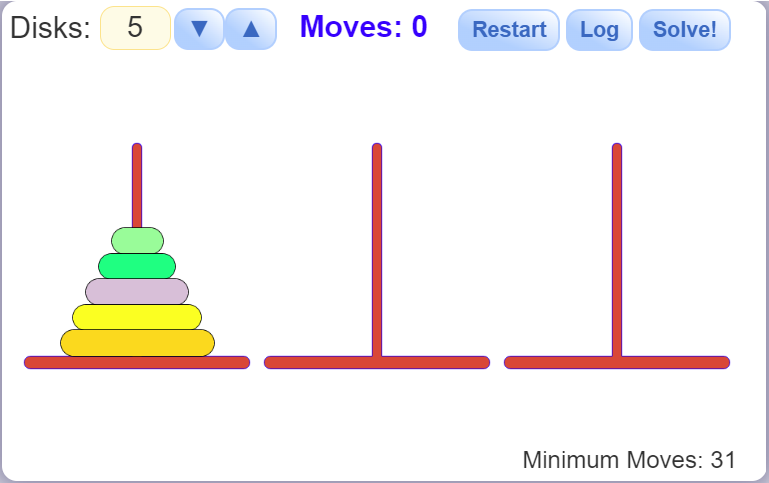
\includegraphics[scale=0.7]{towersOfHanoi_visual.png}
\end{center}

In our class discussion, we established a set of rules in order to then discuss how to represent our functions in code. Below I include both rules as well as repeat some notes on notation 
in order to allow for some context on the second half of this assignment.
\begin{minted}{haskell}
  hanoi 1 x y = move x y 

  hanoi (n+1) x y = 
    hanoi n x (other x y)
    move x y 
    hanoi n (other x y) y
\end{minted}
\begin{itemize}
  \item read \mintinline{haskell}{hanoi n x y} as "move tower of n disks from x to y"
  \item think about how to move a tower of n+1 disks assuming we already know how to move a tower of n disks 
  \item \mintinline{haskell}{hanoi n x y} is a function that takes three arguments: a number n (the number of disks), a number x (encoding the place where the tower is, a number y (encoding the place
  where the tower should go))
  \item \mintinline{haskell}{move x y} is afunction that moves one disk (the topmost disk) from x to y 
  \item \mintinline{haskell}{other x y} denotes the third place which is neither x nor y 
\end{itemize}

Now having laid down some rules for our discussion, we observed that the nature of the Towers of Hanoi problem is recursive given that in order to solve a tower of 4 disks we must first solve 
it with 3 disks and then that requires we solve it for 2 disks and so on. In class we observed the 5 disk tower solution of \mintinline{haskell}{hanoi 5 0 2}. For this assignment, I will write out the 
implementation of this function to cement what we learned about its recursion and logic. 
\begin{minted}{haskell}
  hanoi 5 0 2
    hanoi 4 0 1
      hanoi 3 0 2
        hanoi 2 0 1
          hanoi 1 0 2 = move 0 2
          move 0 1
          hanoi 1 2 1 = move 2 1
        move 0 2
        hanoi 2 1 2 
          hanoi 1 1 0 = move 1 0 
          move 1 2
          hanoi 1 0 2 = move 0 2
      move 0 1
      hanoi 3 2 1 
        hanoi 2 2 0
          hanoi 1 2 1 = move 2 1 
          move 2 0
          hanoi 1 1 0 = move 1 0
        move 2 1
        hanoi 2 0 1
          hanoi 1 0 2 = move 0 2
          move 0 1
          hanoi 1 2 1 = move 2 1
    move 0 2
    hanoi 4 1 2
      hanoi 3 1 0
        hanoi 2 1 2
          hanoi 1 1 0 = move 1 0
          move 1 2
          hanoi 1 0 2 = move 0 2
        move 1 0
        hanoi 2 2 0
          hanoi 1 2 1 = move 2 1
          move 2 0
          hanoi 1 1 0 = move 1 0
      move 1 2
      hanoi 3 0 2
        hanoi 2 0 1
          hanoi 1 0 2 = move 0 2
          move 0 1
          hanoi 1 2 1 = move 2 1
        move 0 2
        hanoi 2 1 2
          hanoi 1 1 0 = move 1 0 
          move 1 2
          hanoi 1 0 2 = move 0 2
\end{minted}

As we can see this is a very lengthy program that relies on its recursive nature to solve the hanoi problem. Now, if we extract from this execution the moves that solve the puzzle (in their right order), we will see that there are 31 moves for the 5-disk tower 
that will solve the problem most efficiently. I say that these are the steps that actually solve the problem since they are the ones that will prompt moving a disk from one tower to another. I will rewrite the steps again below: 
\begin{minted}{haskell}
  move 0 2
  move 0 1
  move 2 1
  move 0 2
  move 1 0
  move 1 2
  move 0 2
  move 0 1 
  move 2 1
  move 2 0
  move 1 0
  move 2 1
  move 0 2
  move 0 1
  move 2 1
  move 0 2
  move 1 0
  move 1 2
  move 0 2
  move 1 0
  move 2 1
  move 2 0
  move 1 0
  move 1 2
  move 0 2
  move 0 1
  move 2 1
  move 0 2
  move 1 0
  move 1 2
  move 0 2
\end{minted}

Now that we have written out the exection, we can also see that the word \mintinline{haskell}{hanoi} appear many times in the computation. I observed the number of occurrences and recorded them in the below table. By looking at the table, we can notice that the
number of occurrences can actually be represented as a formula, for they increase in the same intervals exponentially. Therefore, we can say that with n disks, the number of times the word \mintinline{haskell}{hanoi} appears in the computation is \(2^n - 1\). 
\begin{center}
  \begin{tabular}{|c c|}
    \hline
    n disks & num of hanoi \\
    \hline 
    1 & 1 \\
    \hline 
    2 & 3 \\
    \hline 
    3 & 7 \\
    \hline 
    4 & 15 \\
    \hline 
    5 & 31 \\
    \hline
  \end{tabular}
\end{center}

\subsection{Week 3}
In this week's homework, we are reviewing parsing and context-free grammars. The idea of parsing is immportant to understand as we need it to translate concrete syntax (what we see as more human-readable) into abstract syntax (what a computer will see as more readble). 
In class, we focused on processing abstract syntax in a 2-dimensional view, or what resembles a tree. A context-free grammar is a set of rules that defines a language. One of the examples we used, and the one we will use for the following problems, is a context-free grammar that 
defines arithmetic expressions. In other words, a string is considered to be part of the language defined if it can be dervied from the rules below.
\begin{minted}{haskell}
  Exp -> Exp '+' Exp1
  Exp1 -> Exp1 '*' Exp2
  Exp2 -> Integer 
  Exp2 -> '(' Exp ')'
  Exp -> Exp1
  Exp1 -> Exp2
\end{minted}
Now that we have the rules above, I will write out the derivation trees (aka parse trees or conccrete syntax trees) for the following strings. Note that I numbered the rules above and wrote, in blue, the number of the rule used in each step. The integer definition is implied here so there is no 
number next to those translations. 
\begin{itemize}
  \item 2+1
  \item 1+2*3
  \item 1+(2*3)
  \item (1+2)*3
  \item 1+2*3+4*5+6
\end{itemize}

\begin{center}
  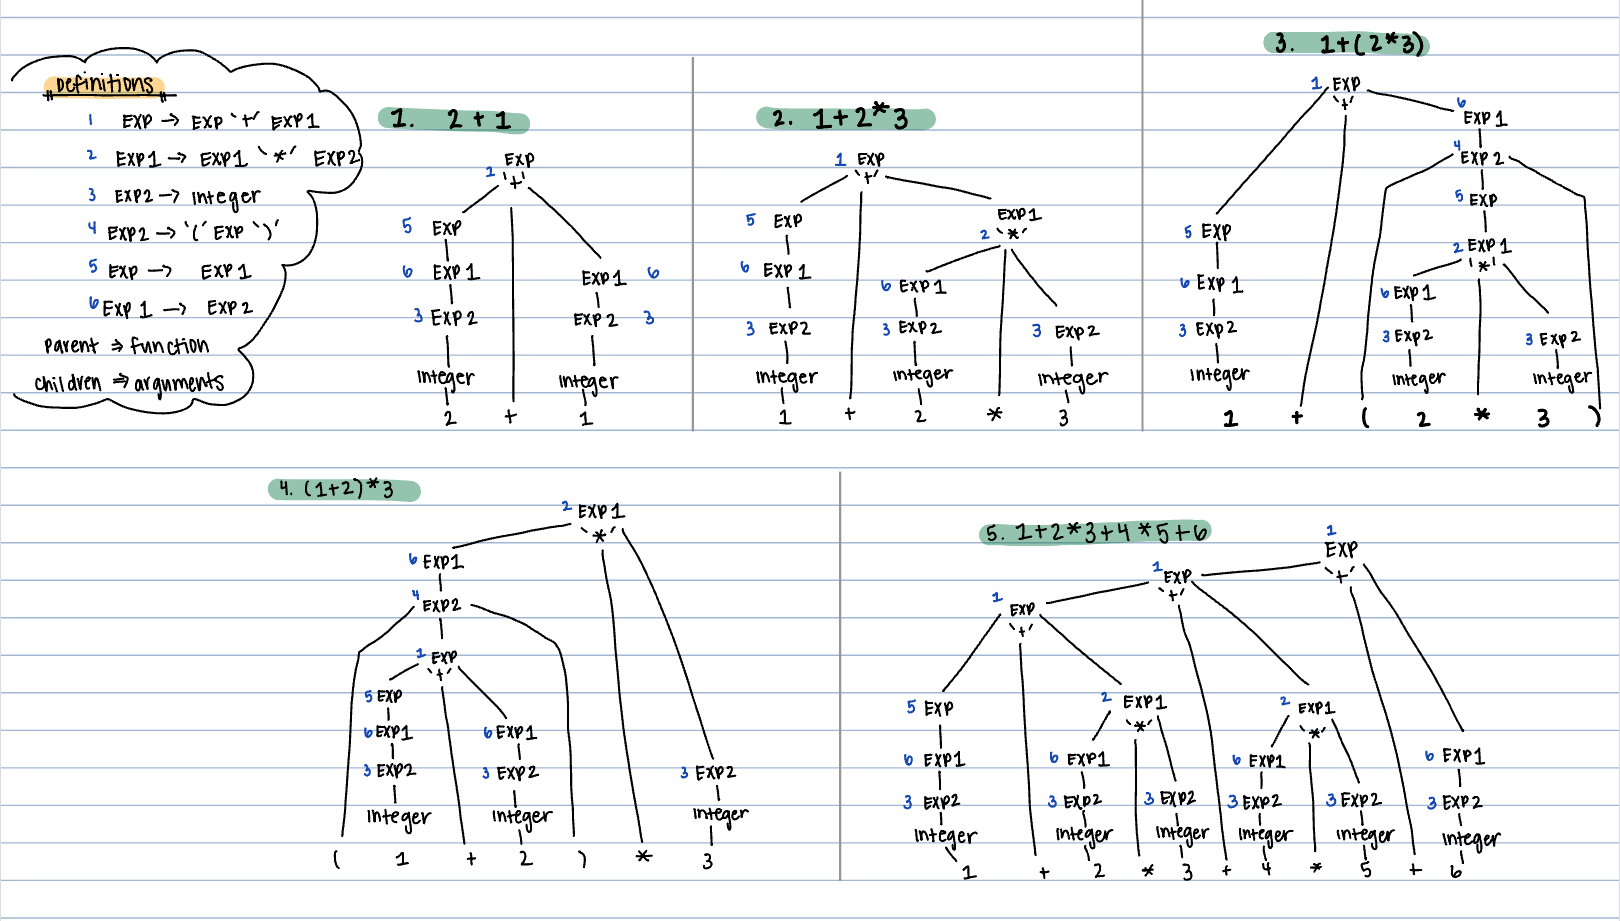
\includegraphics[scale=0.3]{parsing_arithmetic.jpg}
\end{center}


Now that we have covered what the parsing process looks like, we can think bigger. In other words, we can think of a parser that will automatically translate concrete syntax into abstract syntax. Looking at out lesson, we do not attempt to create this type of parser ourselves, but rather 
used a parser generator. In this case, we will input a context-free grammer (like the one above) and the generator will output a parser.

First, I installed the parser generator BNFC, which proved to be a feat of its own. After multiple error messages and researching quests, I was able to successfully download the generator as well as the necessary libraries (alex, happy, etc.). The first commands I used are those described in the 
lecture: 
\begin{minted}{haskell}
  bnfc -m -haskell numbers.cf
  make
  echo "1+2*3" | ./TestNumbers
\end{minted}
This generated some files and then gave me the following output: 
\begin{center}
  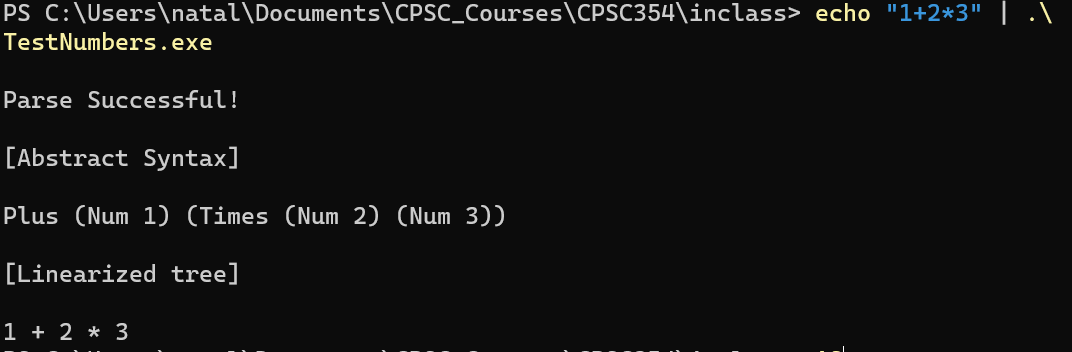
\includegraphics[width=15cm]{bnfc_intro_example.png}
\end{center}

Having run the example successfully, I will now show the outputs for the following given strings: **You will note that these are the same exercises I translated by hand above**
\begin{center}
  2 + 1 \\
  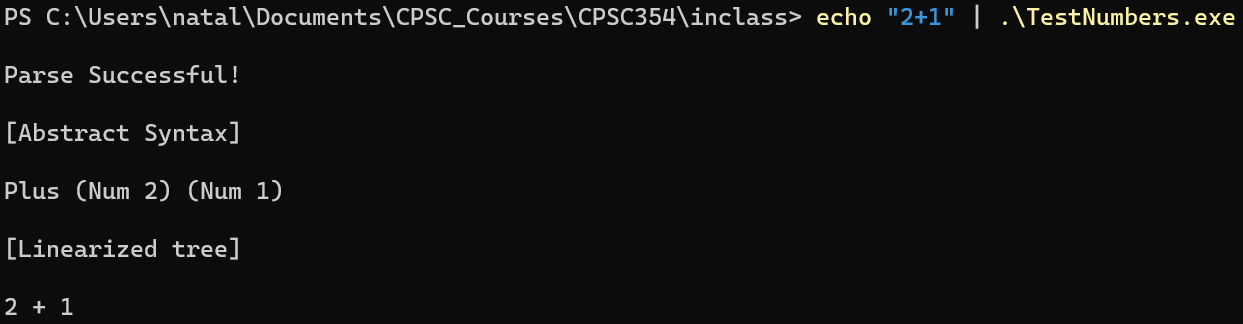
\includegraphics[width=15cm]{bnfc_exercise1a.png}

  1 + 2 * 3\\
  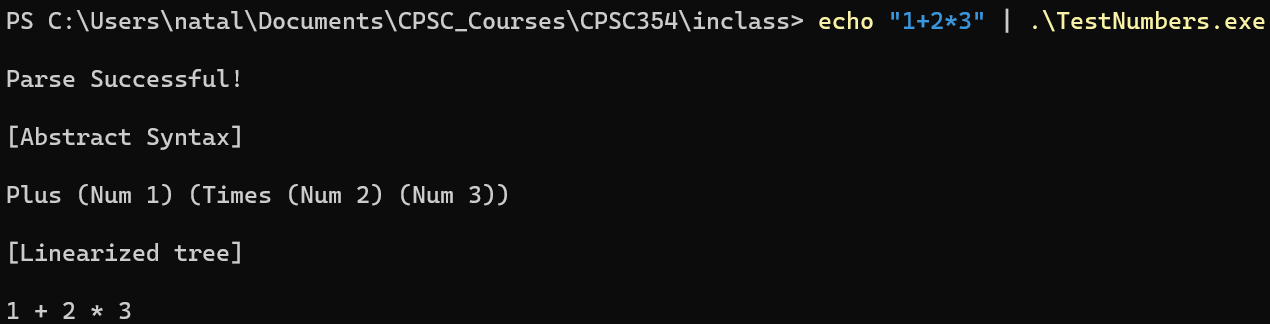
\includegraphics[width=15cm]{bnfc_exercise1b.png}

  1 + ( 2 * 3 )\\
  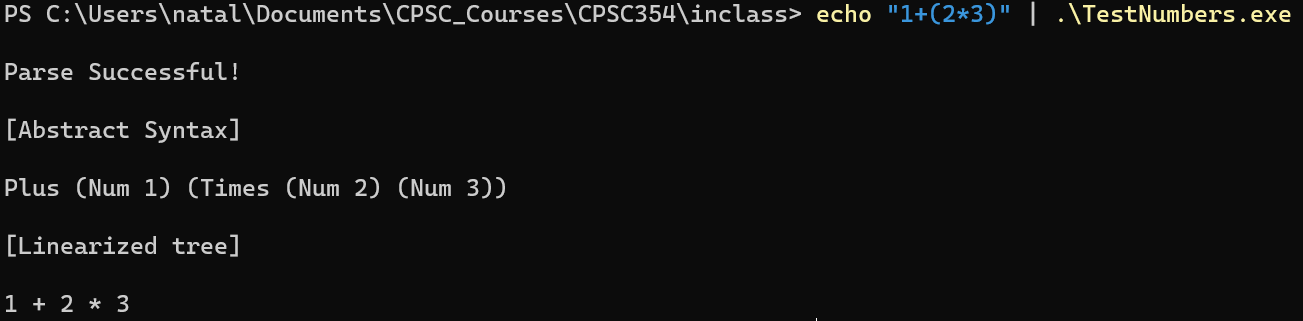
\includegraphics[width=15cm]{bnfc_exercise1c.png}

  ( 1 + 2 ) * 3\\
  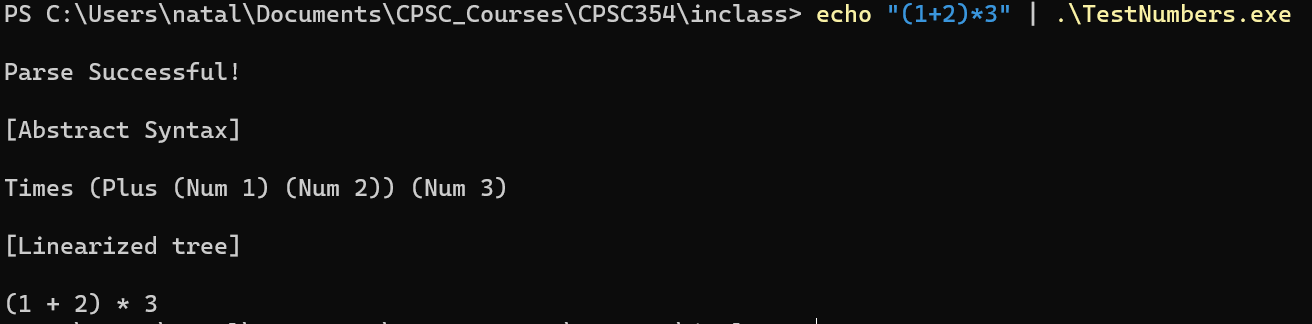
\includegraphics[width=15cm]{bnfc_exercise1d.png}

  1 + 2 * 3 + 4 * 5 + 6\\
  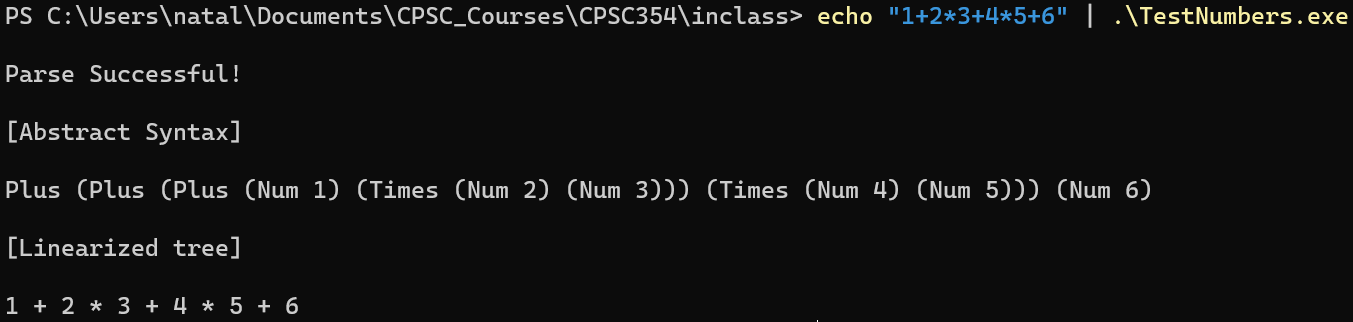
\includegraphics[width=15cm]{bnfc_exercise1e.png}
\end{center}


We can also look at the how the use of paranthesis affects the output. Here we will compare the output between 
\begin{itemize}
  \item 1+2+3
  \item (1+2)+3
  \item 1+(2+3)
\end{itemize}
\begin{center}
  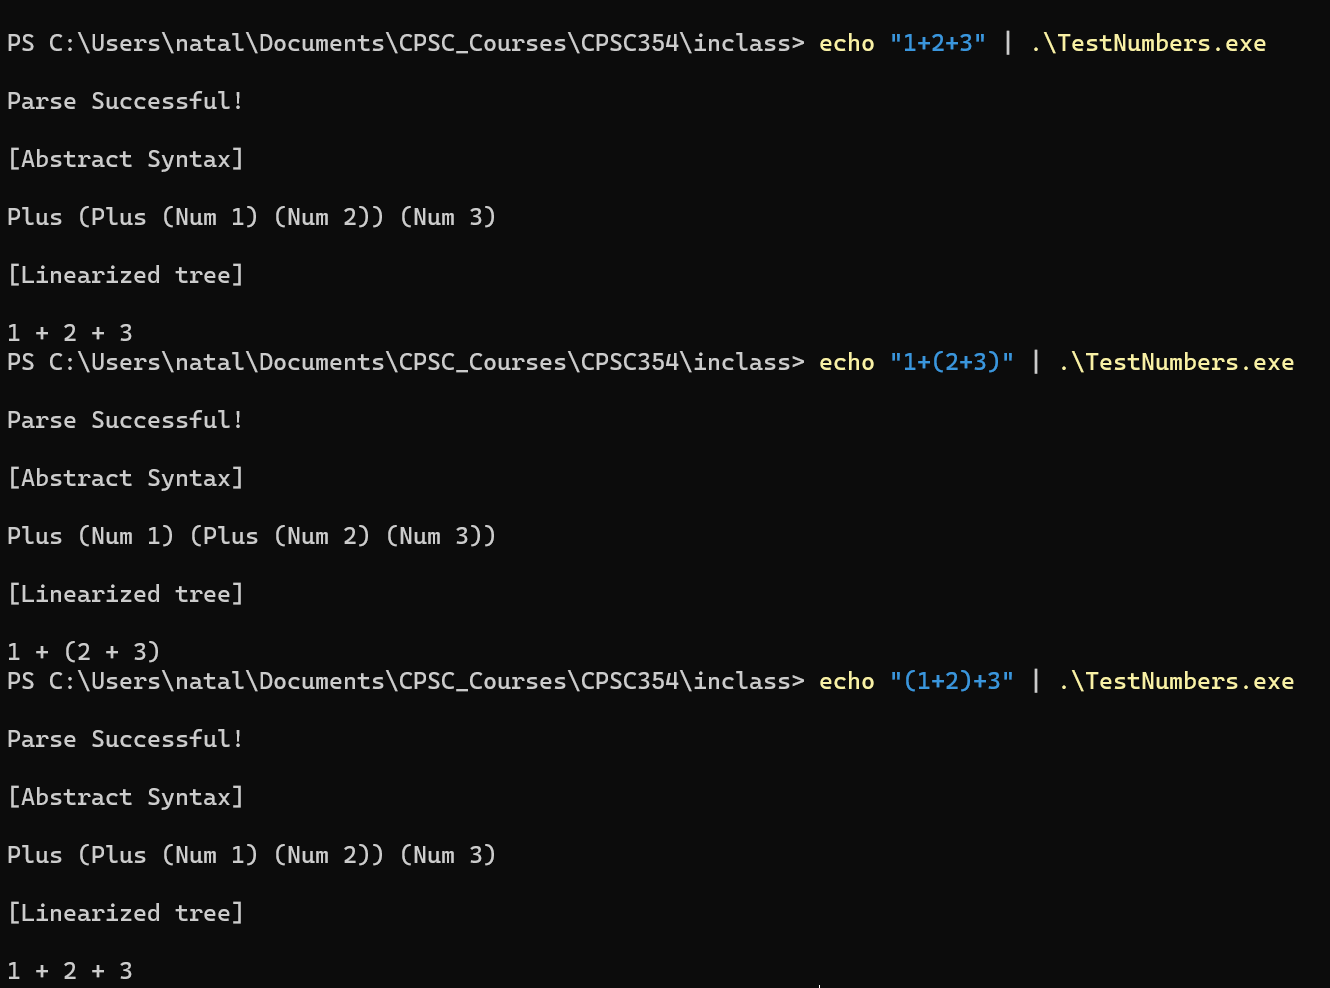
\includegraphics[width=15cm]{bnfc_exercise1f.png}
\end{center}
As you can see, the abstract syntax outputted differs depending on where or if the paranthesis are placed in the expression. The first and last output do yield the same result, implying 
that if the parser is not given any paranthesis, it will prioritize executing from left to right. In this case, the 1 and the 2 are added together first. Therefore, when the 2 and the 3 are 
placed in paranthesis, the abstract syntax changes as the order in which the addition functions are executed also changes. Overall, this homework focused on practicing with and establishing the BNFC 
environment as well as understanding how to convert concrete syntax into abstract syntax. \\

\subsection{Week 4}

\ldots

\section{Conclusions}\label{conclusions}

(approx 400 words) A critical reflection on the content of the course. Step back from the technical details. How does the course fit into the wider world of software engineering? What did you find most interesting or useful? What improvements would you suggest?

\begin{thebibliography}{99}
\bibitem[ALG]{Alg} \href{https://github.com/alexhkurz/algorithm-analysis-2023}{Algorithm Analysis}, Chapman University, 2023.
\end{thebibliography}

\end{document}